\documentclass[a4paper,12pt]{article}
\usepackage[T1]{fontenc}
\usepackage{lmodern}
\usepackage{graphicx}
\graphicspath{ {../img/}, {../front/} }
\usepackage{placeins}
\usepackage[outdir=./]{epstopdf}
\usepackage{subfigure}
\usepackage[english]{babel}
\usepackage{csquotes}
\usepackage[nottoc,numbib]{tocbibind}
\usepackage{pstricks}
\usepackage{amssymb}
\usepackage{lscape}
\usepackage{epsfig} % extra package for .eps graphics usage
\usepackage{pst-grad} % For gradients
\usepackage{pst-plot} % For axes
\usepackage{amsmath} % extra math symbols There are a lot of ams packages
\usepackage{fancyhdr} % to use fancy headers and footers --- requires for most professional docs
\usepackage{watermark} % to include a figure in the background - the front page for example
\usepackage{enumerate} % to enumerate your items in a list with any style
\usepackage{booktabs}
\usepackage[nobottomtitles]{titlesec}
\usepackage{siunitx}
\usepackage{textcomp}
\usepackage{wallpaper}
\usepackage{tabularx}
\usepackage{afterpage}
\usepackage{color}
\definecolor{mygreen}{RGB}{28,172,0}
\definecolor{mylilas}{RGB}{170,55,241}
\usepackage{listings}
\lstset{language=python,%
    %basicstyle=\color{red},
    basicstyle=\footnotesize\ttfamily,
    breaklines=true,%
    morekeywords={matlab2tikz},
    keywordstyle=\color{blue},%
    morekeywords=[2]{1}, keywordstyle=[2]{\color{black}},
    identifierstyle=\color{black},%
    stringstyle=\color{mylilas},
    commentstyle=\color{mygreen},%
    showstringspaces=false,%without this there will be a symbol in the places where there is a space
    numbers=left,%
    numberstyle={\tiny \color{black}},% size of the numbers
    numbersep=9pt, % this defines how far the numbers are from the text     
    emph=[1]{for,end,break},emphstyle=[1]\color{red}, %some words to emphasise
    %emph=[2]{word1,word2}, emphstyle=[2]{style},    
}
\numberwithin{equation}{section}
\numberwithin{figure}{section}
\numberwithin{table}{section}
\usepackage[toc,page,title,titletoc]{appendix}
\usepackage{amsmath}
\usepackage[
backend=bibtex,
style=ieee,
sorting=none
]{biblatex}
\addbibresource{references.bib}

\usepackage[colorlinks=true, linkcolor=blue, citecolor=red, urlcolor=blue]{hyperref}
\parindent=0pt
\parskip=6pt

\renewcommand{\contentsname}{Table of Contents}
%-------------------------------------------------------------------------------
%-------------------------------------------------------------------------------
%-------------------------------------------------------------------------------

\title{\vspace{3 cm}

\includegraphics[scale=0.5]{fronttext}\vspace*{2cm} \\
\Huge{\textsc{
    Exam 1 \\
    Data Analysis} \\ \Large
    REII 424 }
}
		

\author{by:\\ \begin{tabular}{l  r}
    W Bisschoff  & 26217406
\end{tabular}	\\
\\
\textbf{North-West University  Potchefstroom Campus}\\ \\
\begin{Large} 
\begin{tabular}{l l} \\
    Lecturer: & Prof Alwyn Hoffman 
\end{tabular} 
\end{Large} \\
\vspace*{0.8cm}
}

%-------------------------------------------------------------------------------
%-------------------pagestyle stuff & headers & footers ------------------------
%-------------------------------------------------------------------------------
\pagestyle{fancy} % other pagestyles can be used
%\headsep=0.4cm
\headheight=15pt % Have enough space so that the header can fit without warnings
\headwidth=6.7in % the width of the header 
\textwidth=6.6in % the width of the text
\oddsidemargin=0in % the margin indent on odd pagenumbers
\evensidemargin=0in % the margin indent on even pagenumbers

\rhead{\begin{pspicture}(0,0)(0,0)
			
\includegraphics[scale=0.25]{logo_fade.png}
		\end{pspicture}
	}
\chead{} % center header
\lhead{\textbf{\textsf{\footnotesize FACULTY OF ENGINEERING}}} % left header
%-------------------------------------------------------------------------------
%-------------------------------------------------------------------------------
%-------------------------------------------------------------------------------


\lfoot{Exam 1} 


%-------------------------------------------------------------------------------
%-------------------------------------------------------------------------------
%-------------------------------------------------------------------------------
\cfoot{\today} %The current date will be put there
\rfoot{\thepage} %pagenumber
\renewcommand{\headrulewidth}{1pt} % to increase the header or footer line size
\renewcommand{\footrulewidth}{1pt}
%-------------------------------------------------------------------------------
%-------------------------------------------------------------------------------
%-------------------------------------------------------------------------------



%*********************************************************************************
%----------------------------Beginning of the document----------------------------
%*********************************************************************************
\begin{document}
%\sffamily   % include this for sans serif font family
%\fontfamily{pcr} more ways of changing font see: http://tex.loria.fr/general/new/fntguide.html

%\numberwithin{equation}{subsection}
\pagenumbering{roman} % first pages are number in Roman numerals

\ThisULCornerWallPaper{1}{frontcorner.eps}
\maketitle % to display the author and title that was defined earlier

\thispagestyle{empty} % this page should not have header or footers
\pagebreak % break the page here
%-------------------------------------------------------------------------------
%-------------------------------------------------------------------------------
%-------------------------------------------------------------------------------

%\section*{Abstract}
%A DC motor needs to be controlled within a set of specifications. The DC motor is characterised an a transfer function is obtained. A PI controller is designed and then implemented with an Arduino. 
%\pagebreak


\tableofcontents

\newpage{}
{
\let\oldnumberline\numberline%
\renewcommand{\numberline}{\figurename~\oldnumberline}%
\listoffigures
}
\newpage{}
{
\let\oldnumberline\numberline%
\renewcommand{\numberline}{\tablename~\oldnumberline}%
\listoftables
}



% The beginning of the sections
\newpage
\pagenumbering{arabic}

\section{Question 1}
\subsection{Question 1 a, b}
A folder of XML files are read into a Pandas Dataframe. The first level of fields are specified, assnap well as the fields inside the customs responses fields. \par 
The tags are iterated through and placed in temporary dataframes to be later merged into one. Customs responses items are also iterated through and placed into another dataframe to be placed inside the upper dataframe. \par 
This is done with the function in Listing~\ref{readxml}. \par 
This function is called for each file and placed in a seperate process to speed up the process in Listing~\ref{readall}. \par 
The output can be seen in Table~\ref{tab:readxml}.

\begin{table}[!htb]
    \centering
    \caption{File Processing Output}
    \label{tab:readxml}
    \begin{tabular}{lr}
    \toprule
    Time & 0:08:40.084965 \\
    Number of files & 179\\
    Number of entries & 48520\\\bottomrule
    \end{tabular}
\end{table}

The first 5 entries of the dataframe can be seen in Fig.~\ref{fig:1a}. There are 25 columns in total, most of which is out of frame.

\begin{figure}[!htb]
    \centering
    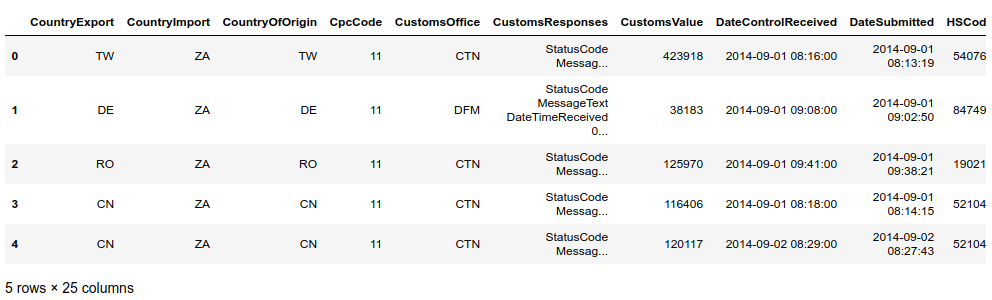
\includegraphics[width=0.8\linewidth]{1a.png}
    \caption{The Resulting Dataframe}
    \label{fig:1a}
\end{figure}
\FloatBarrier

An example of the CustomsResponses dataframe is shown in Fig.~\ref{fig:1a2}.
\begin{figure}[!htb]
    \centering
    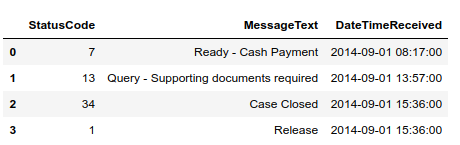
\includegraphics[width=0.6\linewidth]{1a2.png}
    \caption{The First Entry's CustomsResponses DataFrame}
    \label{fig:1a2}
\end{figure}
\FloatBarrier

The length of the dataframe is calculated as 48215. \par 

The number of customs responses are calculated by applying the \emph{len} function to the inner dataframe for every row:
\lstset{language=Python} 
\begin{lstlisting}
    csv_data['NoCustomsResponses'] = (csv_data['CustomsResponses']).apply(len)
\end{lstlisting}

\begin{figure}[!htb]
    \centering
    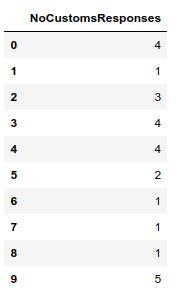
\includegraphics[width=0.25\linewidth]{1b.png}
    \caption{Number of Customs Responses for the First Ten Entries}
    \label{fig:1b}
\end{figure}
\FloatBarrier

\clearpage
\subsection{Question 1 c}
There were no duplicates found after comparing the length of the dataframe to the length of the dataframe with dropped duplicates. \par 
The dataframe is sorted by the submitted dates. as in Fig.~\ref{fig:1c}. Only two columns are shown. \par 
The number of entries did not change.
\lstinputlisting[language=Python, firstline=139, lastline=141]{../../codes.py}

\begin{figure}[!htb]
    \centering
    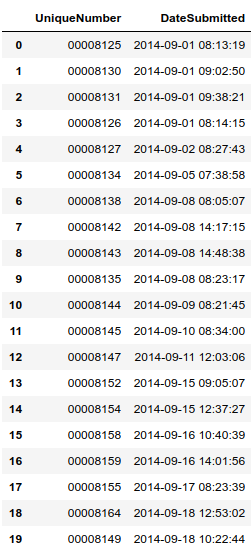
\includegraphics[width=0.25\linewidth]{1c.png}
    \caption{First 20 Entries of the Sorted Dataframe}
    \label{fig:1c}
\end{figure}
\FloatBarrier


\clearpage
\subsection{Question 1 d}

Categories were created for each transaction from the HS codes. A new function was created that takes a code and searches for the appropriate category within a created dictionary with the first two characters of the code. \par 
This was also done with multi processing and the time was measured to compare the processing speed. \par 
The first twenty results of Listing~\ref{categorize} can be seen in Fig.~\ref{fig:1d}.

\begin{figure}[!htb]
    \centering
    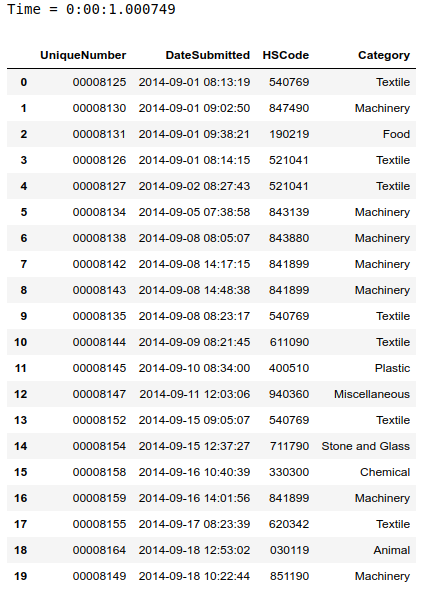
\includegraphics[width=0.55\linewidth]{1d.png}
    \caption{First Twenty Entries of the Dataframe with Added Categories}
    \label{fig:1d}
\end{figure}
\FloatBarrier

\subsection{Question 1 e}

The durations were calculated with Listing~\ref{duration}. Entries with invalid durations were removed. \par 
The other fields were generated with Listing~\ref{codes}. Sets of codes for each field was created. From the inner customs response dataframe, a set of codes was generated for every transaction. These codes are then compared to those for the fields to generate the output variables. \par 
The calendar month is also calculated here for future use. \par
The first twenty entires with the output variables are shown in Fig.~\ref{fig:1e}.

\begin{figure}[!htb]
    \centering
    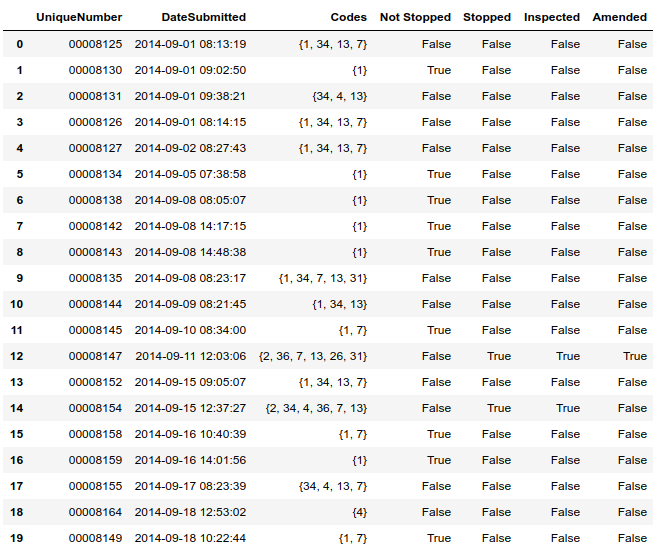
\includegraphics[width=0.65\linewidth]{1e.png}
    \caption{First Twenty Entries of the Dataframe with Added Output Variables}
    \label{fig:1e}
\end{figure}
\FloatBarrier

\newpage
\subsection{Question 1 f}

An array with all the categories is created. Through iterations the dataframe groups by the category and counts the number of transactions as well as the number of categories. The code can be seen in Listing~\ref{count}. 


\begin{figure}[!htb]
    \centering
    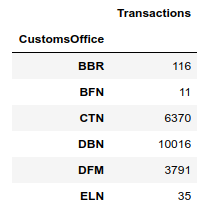
\includegraphics[width=0.25\linewidth]{1f.png}
    \caption{First Six Entries of the Number of Transactions for each Customs Office}
    \label{fig:1f}
\end{figure}
\FloatBarrier

\begin{figure}[!htb]
    \centering
    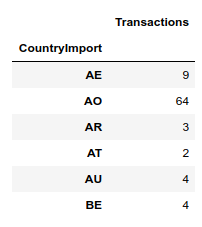
\includegraphics[width=0.25\linewidth]{1f2.png}
    \caption{First Six Entries of the Number of Transactions for each Country of Import}
    \label{fig:1f2}
\end{figure}
\FloatBarrier
\begin{figure}[!htb]
    \centering
    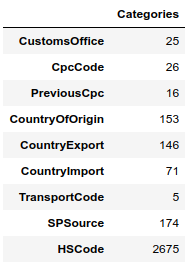
\includegraphics[width=0.25\linewidth]{1f3.png}
    \caption{The Number of Sub Categories per Category}
    \label{fig:1f3}
\end{figure}
\FloatBarrier

\section{Question 2}
\subsection{Question 2 a, b, c}

Dictionaries were created to hold the number of transactions, document requests and fractions for each category. The dataframe is manipulated to show grouped info for each calendar month for each sub-category, for each category. \par 
This is then repeated for only transactions that requested additional documents. \par
These two new dataframes are then divided to create a fraction of document requests. \par 
A rolling mean is applied to the columns in the new dataframe. \par 
The output of Listing~\ref{requests} is shown in the following figures.

\begin{figure}[!htb]
    \centering
    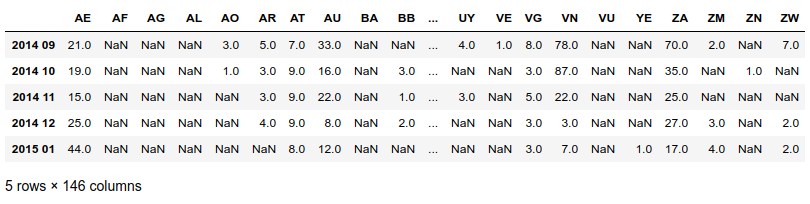
\includegraphics[width=0.85\linewidth]{2a.png}
    \caption{First Five Entries of Monthly Entries by Export Country}
    \label{fig:2a}
\end{figure}
\FloatBarrier

\begin{figure}[!htb]
    \centering
    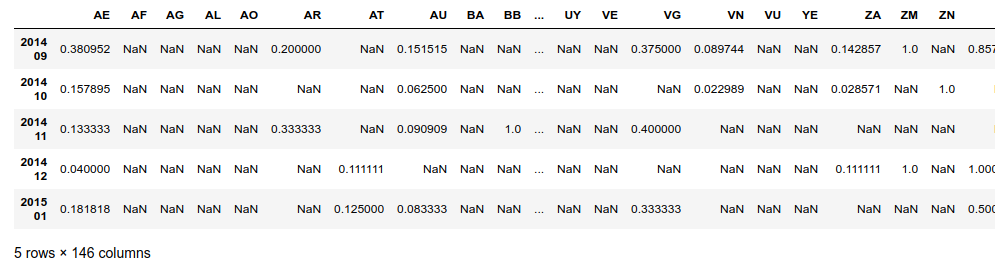
\includegraphics[width=0.85\linewidth]{2a2.png}
    \caption{First Five Entries of Fractions of Document Requests by Export Country}
    \label{fig:2a2}
\end{figure}
\FloatBarrier

\begin{figure}[!htb]
    \centering
    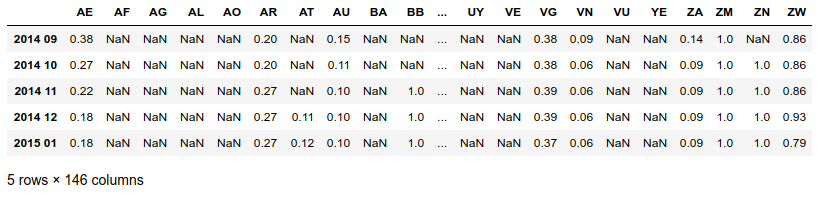
\includegraphics[width=0.85\linewidth]{2a3.png}
    \caption{First Five Entries of Accumulated Fractions of Document Requests by Export Country}
    \label{fig:2a3}
\end{figure}
\FloatBarrier

\begin{figure}[!htb]
    \centering
    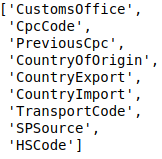
\includegraphics[width=0.25\linewidth]{2a4.png}
    \caption{List of All Categories that Declarations were Calculated For}
    \label{fig:2a4}
\end{figure}
\FloatBarrier


\subsection{Question 2 d}

Accumulated fractions are allocated to each transaction per category through Listing~\ref{getval}. A new dataframe is created with the values. This is also appended to the main dataframe. \par 
Fig.~\ref{fig:2d} shows the dataframe with category values for the first ten transactions.

\begin{figure}[!htb]
    \centering
    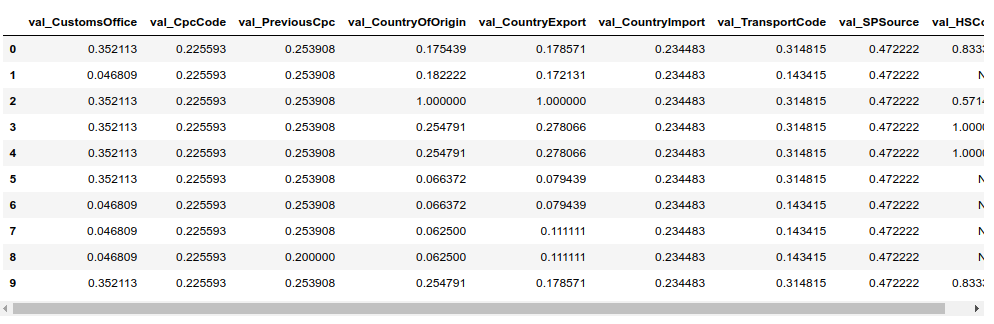
\includegraphics[width=0.85\linewidth]{2d.png}
    \caption{First Ten Entries of Transaction Category Values}
    \label{fig:2d}
\end{figure}
\FloatBarrier

\subsection{Question 2 e}
The following code is used to calculate the Pearson correlation coefficients. The dataframe's built in \emph{corr()} function is used. 
\lstinputlisting[language=Python, firstline=358, lastline=359]{../../codes.py}

Fig.~\ref{fig:2e} shows the coefficients for each category. The bar plot is shown in Fig.~\ref{fig:corrcoeff}

\begin{figure}[!htb]
    \centering
    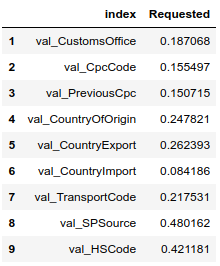
\includegraphics[width=0.25\linewidth]{2e.png}
    \caption{Pearson Correlation Coefficients for each Category}
    \label{fig:2e}
\end{figure}
\FloatBarrier


\begin{figure}[!htb]
    \centering
    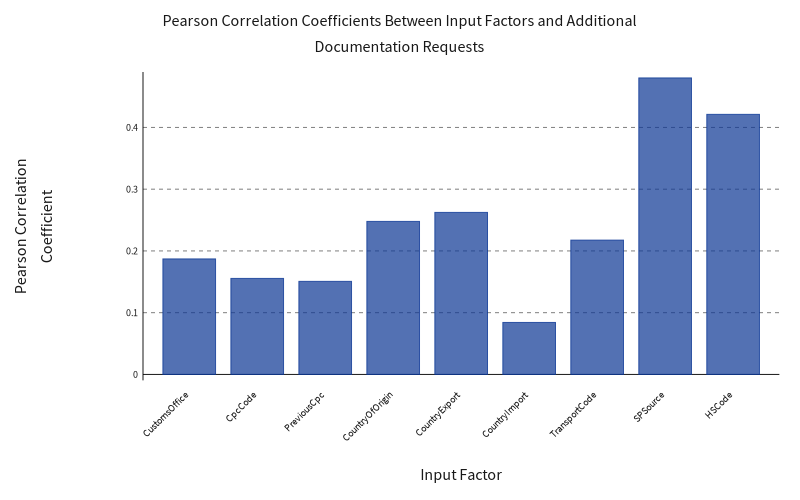
\includegraphics[width=0.95\linewidth]{../../corrcoeff.png}
    \caption{Bar Graph of Pearson Correlation Coefficients}
    \label{fig:corrcoeff}
\end{figure}
\FloatBarrier

\section{Question 3}
\subsection{Question 3 a}
Sklearn is used to split data between training sets and testing sets.
\lstinputlisting[language=Python, firstline=432, lastline=434]{../../codes.py}

\subsection{Question 3 b}
To ensure a 50:50 split between transactions that request additional documents and those that do not, data needs to be duplicated. Transactions that request documents are added until the number of entries is equal or larger than the non-requests. 
\lstinputlisting[language=Python, firstline=421, lastline=424]{../../codes.py}

\subsection{Question 3 c}
The correlation coefficients are sorted and the largest three categories are used to plot the number of document requests against the request fraction values. The results of the following snippet is shown in the following figures. \par 
From the graphs it seems that Export Country has the best ability to identify additional document request cases, followed by SP Source and then HS Code.

\lstinputlisting[language=Python, firstline=440, lastline=448]{../../codes.py}


\begin{figure}[!htb]
    \centering
    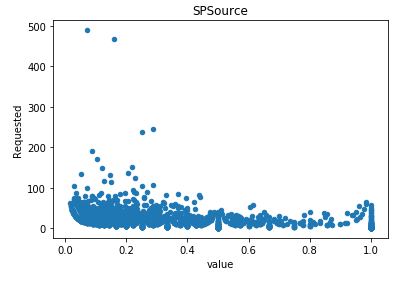
\includegraphics[width=0.4\linewidth]{3c.png}
    \caption{Number of Document Requests vs Fraction of Document Requests of SP Source}
    \label{fig:2e}
\end{figure}
\FloatBarrier

\begin{figure}[!htb]
    \centering
    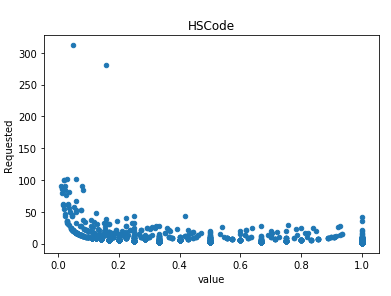
\includegraphics[width=0.4\linewidth]{3c2.png}
    \caption{Number of Document Requests vs Fraction of Document Requests of HS Code}
    \label{fig:2e}
\end{figure}
\FloatBarrier
\begin{figure}[!htb]
    \centering
    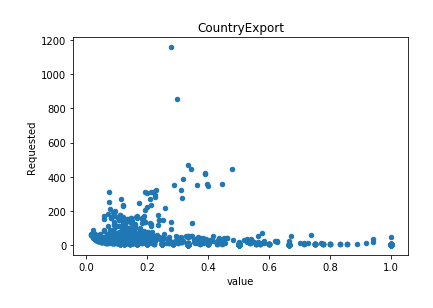
\includegraphics[width=0.4\linewidth]{3c3.png}
    \caption{Number of Document Requests vs Fraction of Document Requests of Export Country}
    \label{fig:2e}
\end{figure}
\FloatBarrier


\section{Question 4}
\subsection{Question 4 a}
Sklearn is used to create a Linear Regression model. The regression coefficients are shown in Table~\ref{tab:reg}.

\lstinputlisting[language=Python, firstline=477, lastline=481]{../../codes.py}

\begin{table}[!htb]
    \centering
    \caption{Linear Regression Coefficients}
    \label{tab:reg}
    \begin{tabular}{lr}
    \toprule
    Category & Coefficient \\\midrule
    CustomsOffice & 0.08299145\\
    CpcCode & 0.08299145\\
    PreviousCpc & 0.55039948\\
    CountryOfOrigin & -0.03845656\\
    CountryExport & 0.13658853\\
    CountryImport & 0.14750978\\
    TransportCode & 0.28401459\\
    SPSource & 0.50424546\\
    HSCode & 0.52598281\\
    Number of entries & 0.39340001\\\bottomrule
    \end{tabular}
\end{table}

\subsection{Question 4 b}

Listing~\ref{predict} iterates through multiple threshold values. Predictions are made with linear regression and converted into binary values with the threshold. A dataframe is then generated that contains the fraction of correct predictions for all observations, observations where the target is 1 and observations where the target is 0, for each threshold value. \par 
Fig.~\ref{fig:4b} shows the first five values of this dataframe.

\begin{figure}[!htb]
    \centering
    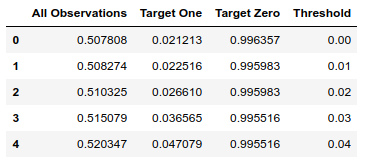
\includegraphics[width=0.4\linewidth]{4b.png}
    \caption{Prediction Accuracy for Different Targets per Threshold Value}
    \label{fig:4b}
\end{figure}
\FloatBarrier

The plot of the above dataframe can be seen in Fig.~\ref{fig:predict}. 

\begin{figure}[!htb]
    \centering
    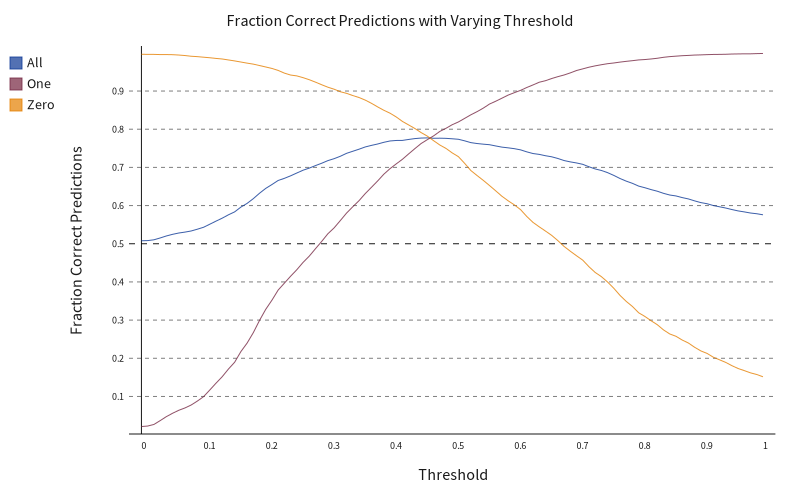
\includegraphics[width=0.95\linewidth]{../../predict.png}
    \caption{Plot of Prediction Accuracy for Different Targets per Threshold Value}
    \label{fig:predict}
\end{figure}
\FloatBarrier

\subsection{Question 4 c}

\lstinputlisting[language=Python, firstline=560, lastline=563]{../../codes.py}

\begin{table}[!htb]
    \centering
    \caption{Threshold Values to Predict Specific Target Percentages}
    \label{tab:predict}
    \begin{tabular}{cccc}
    \toprule
    Threshold & All Observations & Target Value 1 & Target Value 0 \\\midrule
    0.29 & 0.710856	& 0.506048 & 	0.916488 \\	
    0.49 & 0.776069	& 0.802382 & 	0.749650	 \\	
    0.61 & 0.745910	& 0.901842 & 	0.589351 \\	
    0.69 & 0.714446	& 0.947525 & 	0.480430 \\\bottomrule
    \end{tabular}
\end{table}


\clearpage
\begin{appendices}
\section{Code}
\subsection{Question 1}
\subsubsection{Read XML Function}
\label{readxml}
\lstinputlisting[language=Python, firstline=27, lastline=68]{../../codes.py}

\newpage
\subsubsection{Read All Files}
\label{readall}
\lstinputlisting[language=Python, firstline=74, lastline=92]{../../codes.py}

\newpage
\subsubsection{Categorize}
\label{categorize}
\lstinputlisting[language=Python, firstline=149, lastline=172]{../../codes.py}

\newpage
\subsubsection{Calculate Durations}
\label{duration}
\lstinputlisting[language=Python, firstline=180, lastline=197]{../../codes.py}

\newpage
\subsubsection{Generate Output Variables}
\label{codes}
\lstinputlisting[language=Python, firstline=203, lastline=251]{../../codes.py}

\newpage
\subsubsection{Count Transactions per Category}
\label{count}
\lstinputlisting[language=Python, firstline=257, lastline=266]{../../codes.py}

\newpage
\subsection{Question 2}
\subsubsection{Fractions of Requests for Additional Documents}
\label{requests}
\lstinputlisting[language=Python, firstline=280, lastline=299]{../../codes.py}

\newpage
\subsubsection{Generate Output Variables From Accumulated Document Request Fractions}
\label{getval}
\lstinputlisting[language=Python, firstline=307, lastline=337]{../../codes.py}
\newpage
\subsection{Question 4}
\subsubsection{Predict Values with Varying Thresholds}
\label{predict}
\lstinputlisting[language=Python, firstline=307, lastline=337]{../../codes.py}
\end{appendices}
\end{document}